\section{Introduction}

La Grille.

Ce monde de programmes, régi par des programmes pour les programmes,
est dirigé d'un pointeur de fer par Clu. Chargé de concevoir un monde
parfait, Clu fait régner la terreur, désactivant sans pitié\footnote{Le fameux supplice de la planche à Clu.} tout programme faisant un pas de travers\footnote{Tu fais une \emph{segfault}, t'es mort.}.

Depuis qu'il connaît l'existence du monde réel, Clu cherche à tout prix à s'y infiltrer, pour y porter sa vision du monde parfait. La seule passerelle entre son monde numérique et le nôtre est le Portail, dont l'ouverture nécessite des quantités astronomiques d'énergie.

Pour arriver à ses fins, il organise donc des jeux sur la Grille pour que les programmes s'affrontent deux à deux. Cela lui permet à la fois de déterminer les éléments les mieux conçus au moyen d'un classement, et de recueillir de l'énergie.

Prologin, une organisation secrète visant à sauver la Terre d'une destruction imminente, a repéré les 100 meilleurs concepteurs\footnote{Les 100 les moins mauvais, disons.} à travers toute la France. Pensant qu'ils allaient participer à la finale d'un concours d'informatique\footnote{Ha ha, non mais quels naïfs !}, ils ont en réalité été envoyés dans la Grille en mission d'infiltration \footnote{Et non, cette fois, ce n'est pas en vous suicidant que vous retournerez dans le monde réel. Bien essayé.}.

Vous êtes donc à présent des programmes.

\newpage

        \subsection{Votre mission}
\citationTron{"What am I supposed to do?"\\
"Survive."}

Vous devez relier des sources d'énergie à des consommateurs, en fonction des teneurs des premières et des besoins des dernières, au moyen d'une succession de traînées contiguës extensibles laissées par des lumicycles\footnote{Vous pouvez relire la phrase.}.

Lors d'une partie, deux programmes s'affronteront, agissant à tour de rôle. Au bout de 150 tours, celui qui aura obtenu le plus de points de la Grille sera le vainqueur.

Attention. C'est lui ou vous\footnote{C'est dramatique, mais voyez le bon côté des choses : vous aurez une plus grosse part de gâteau lundi midi si votre adversaire ne revient pas dans le monde réel.}.

\subsection{La Grille}

\citationTron{The Grid. A digital frontier. I tried to picture clusters
          of information as they moved through the computer. What did they
          look like? Ships, motorcycles? Were the circuits like freeways? I
          kept dreaming of a world I thought I'd never see. And then, one
          day, I got in\ldots{}}

Vous vous battrez sur la Grille, environnement numérique carré se découpant en 30 cases par 30 cases, sur lesquelles sont notamment éparpillées les précieuses sources d'énergie et les consommateurs.

\newpage
\section{Les règles}
\citationTron{Patience, Sam Flynn. All of your questions will be answered soon.}

Un lumicycle est une moto qui laisse une traînée de lumière.

Vous êtes-vous déjà demandé pourquoi les traînées\footnote{Ne jouez pas sur les mots, hein, on a déjà assez peu de filles comme ça.} des motos sont dangereuses ? C'est parce qu'elles véhiculent de l'énergie !

        \subsection{Les traînées de lumière}

À chaque tour, vous interagirez avec des traînées de lumière sur la Grille. Vous pouvez en déplacer les extrémités, les couper, les fusionner, ou les concentrer en un point.

Deux traînées de lumière ne peuvent pas se croiser sur une case normale.

Soyez vigilants, tout ordre vous coûtera un PA (point d'action), et ces PA sont rares\footnote{Comme dirait Ken le survivant, « Décidément les temps comme les œufs sont durs. »}. La Grille vous en donne un certain
nombre en début de tour, mais récupérera les PA inutilisés en fin de tour.

\subsection{La Grille}

\citationTron{In there is a new world! In there is our future! In
          there is our destiny!}

Sur la Grille, vous pouvez rencontrer :

\begin{itemize}
  \item des \textbf{obstacles} 
\includegraphics[width=4mm]{../data/graphics/terrain-obstacle.png} ;
  \item un \textbf{bonus} que vous pouvez ramasser en vous déplaçant dessus ;
  \item un \textbf{point de croisement} 
\includegraphics[width=4mm]{../data/graphics/terrain-point_croisement.png} : sur ces cases, il est
    possible pour au moins deux traînées de se croiser sans dommage.
  \item une \textbf{unité d'énergie} : soit une
    source d'énergie, soit un consommateur.
\end{itemize}

Sans oublier les traînées de votre adversaire, qui se comportent comme des obstacles.

\subsection{Les unités d'énergie}

Votre objectif est de transférer un maximum
d'énergie des sources vers les consommateurs, et éventuellement d'empêcher votre
adversaire de le faire.

\subsubsection{Transfert d'énergie}

Pour vous relier à une source d'énergie, il suffit qu'une des traînées que vous commandez touche l'une des 8 cases\footnote{Et non 4.} autour de celle-ci. Il en va de même pour les consommateurs. Deux traînées peuvent se transmettre de l'énergie si on peut sauter de l'une à l'autre en empruntant une des 4 directions\footnote{Et non 8.}. Une source reliée à au moins un consommateur par vos traînées seulement est dite \emph{active}.

Chaque unité d'énergie est caractérisée par une valeur $v$. Si elle est positive, il s'agit d'une source de \emph{teneur} $v$. Si elle est négative, il s'agit d'un consommateur de \emph{besoin} $-v$. Si cette valeur est nulle, l'unité est dite \emph{épuisée}.

À la fin du tour, le transfert issu d'une liaison entre des sources de teneur totale $T$ (somme des teneurs) et des consommateurs de besoin total $B$ vous rapportera $\min(T, B)$ points. Il est donc de votre intérêt de relier les sources les plus abondantes aux consommateurs les plus affamés.

\begin{figure}[!h]
\centering
\begin{tabular}{c|c}
    
\includegraphics{../data/graphics/source_energie-on-producteur.png}
& 
\includegraphics{../data/graphics/source_energie-off-producteur.png}\\
Point d'énergie non épuisé & Point d'énergie épuisé\\
\hline
    
\includegraphics{../data/graphics/source_energie-on-consommateur.png}
& 
\includegraphics{../data/graphics/source_energie-off-consommateur.png}\\
Consommateur non épuisé & Consommateur épuisé\\
\hline
\raisebox{3mm}{
\includegraphics[width=0.2\linewidth]{404.pdf}} & 
\includegraphics[width=0.2\linewidth]{orga.png}\\
Organisateur non épuisé & Organisateur épuisé
\end{tabular}
\caption{Les différentes unités d'énergie}
\end{figure}

\subsubsection{Affaiblissement et régénération des unités}

La \emph{charge} d'une traînée est le nombre d'unités directement reliées à celle-ci.

À chaque fin de tour, après que les 2 programmes ont joué, chaque source d'énergie active (resp. consommateur actif) diminue sa teneur (resp. besoin) de la somme des charges des traînées qui lui sont directement reliées\footnote{Si vous n'avez pas compris, demandez à un gentil organisateur (ils se font rares, en cette saison) et priez pour qu'il ne vous dise pas le contraire.}.

Les sources inactives (resp. consommateurs inactifs), quant à elles, augmentent leur teneur (resp. besoin) d'un point.

\begin{figure}[h]
\centering
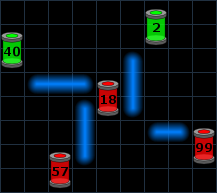
\includegraphics{transfert.png}\hspace{5mm}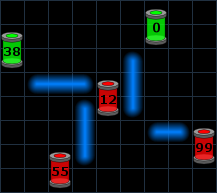
\includegraphics{transfert2.png}
\caption{Un exemple de transfert, avant puis après la fin du tour}
\label{fig:transfert}
\end{figure}

Ici, 4 unités d'énergie sont reliées (le consommateur de besoin 99 n'appartient pas au réseau car les traînées ne peuvent véhiculer de l'énergie en diagonale), le nombre de points obtenu est : $\min(40 + 2, 18 + 57) = 42$\footnote{Vous voyez, ce n'était même pas la peine de vous poser la question.}. Le consommateur de besoin 99 n'est pas relié à une source, donc il n'est pas affaibli à la fin du tour.

\subsection{L'interaction avec la Grille}
\citationTron{This is Blue Leader to Blue Bikes. Run these guys into your jet walls.}

\subsubsection{Déplacement d'une traînée}

Une traînée de lumière a une certaine \emph{intensité}, qui représente le nombre maximum de cases sur lesquelles elle peut s'étendre.

Vous pouvez déplacer une traînée à partir d'une de ses deux extrémités en direction des 4 points cardinaux.

\begin{figure}[h]
\centering
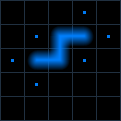
\includegraphics{positions.png}
\caption{Différents déplacements possibles}
\end{figure}

Lorsqu'une traînée n'est pas complètement déployée, le déplacement d'une de ses extrémités laisse l'autre extrémité immobile.

\begin{figure}[h]
\centering

\includegraphics{deplacement1.png}\hspace{5mm}
\includegraphics{deplacement2.png}
\caption{Déplacement d'une traînée de longueur 4 d'intensité 5}
\end{figure}

Lorsqu'une traînée est complètement déployée, les deux extrémités se déplacent.

\begin{figure}[h]
\centering

\includegraphics{deplacement3.png}\hspace{5mm}
\includegraphics{deplacement4.png}
\caption{Déplacement d'une traînée de longueur 5 d'intensité 5}
\end{figure}

\subsubsection{Autres actions}

Vous pouvez \textbf{couper} une traînée entre deux positions adjacentes et répartir l'intensité comme vous le souhaitez entre les deux traînées résultantes, que vous pouvez contrôler indépendamment.

Inversement, il vous est possible de \textbf{fusionner} deux traînées contiguës\footnote{« contiguës », hein.}. La traînée résultante aura pour intensité la somme de leurs intensités.

\begin{figure}[h]
\centering
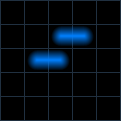
\includegraphics{contigues.png}\hspace{5mm}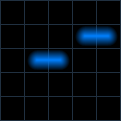
\includegraphics{noncontigues.png}
\caption{Deux traînées contiguës à gauche, non contiguës à droite.}
\end{figure}

Enfin, vous pouvez \textbf{concentrer} toute une traînée en un seul point, sans altérer son intensité.

\newpage
\section{Les bonus}\label{bonus}
\citationTron{Now for some real user power.}

Les bonus qui peuvent apparaître sur la carte sont les suivants.
\begin{itemize}
\item \textbf{point de croisement} 
\includegraphics[width=5mm]{../data/graphics/bonus-bonus_croisement.png} : vous permet de placer un point de croisement sur n'importe quelle case de la Grille ;
\item \textbf{régénération} 
\includegraphics[width=5mm]{../data/graphics/bonus-bonus_regeneration.png} : restaure la teneur maximale d'une source ou le besoin maximal d'un consommateur ;
\item \textbf{allongement} 
\includegraphics[width=5mm]{../data/graphics/bonus-plus_long.png} : augmente l'intensité d'une traînée ;
\item \textbf{PA+} 
\includegraphics[width=5mm]{../data/graphics/bonus-plus_pa.png} : augmente votre nombre de points d'action.
\end{itemize}\bigskip

Vous pouvez les utiliser quand vous le souhaitez\footnote{Avant la fin des 150 tours, c'est mieux.}.

\section{Conclusion}

\citationTron{End of Line, man.}

À l'issue d'un tournoi sans merci de 36 heures, un classement sera établi. Clu, élitiste, vouera une confiance aveugle aux 10 meilleurs programmes. Or, être puissant ne veut pas dire qu'on est de confiance\footnote{Prenez exemple sur le gouvernement français.}. Ainsi, l'Équipe des Dix rejoindra le monde réel, en compagnie de Clu. Leur tâche consistera ensuite à le noyer\footnote{Clu ne sait pas nager, il est un peu rouillé.} dans la zone de décontamination\footnote{Communément appelée \emph{piscine de mousse}.}. Enfin, ils passeront un entretien avec le Conseil des Quatre pour expliquer les stratégies qu'ils auront utilisées. Quant aux 90 autres, ils seront condamnés à perdre au jeu éternellement\footnote{Je sais. C'est terrible.}.

En bref, le sort de la Terre est entre vos mains.

\vspace{5cm}

\noindent
« Je trouve toujours toute cette compétition dégueulasse »\\
— Valérie Lemercier